\documentclass{beamer}
\usepackage{hyperref}
\usepackage{parskip}
\usepackage{verbatim}
\usepackage{tabularx}
\usepackage{amsmath}
% \usetheme{Madrid}
\usetheme{Boadilla}
% \usetheme{Montpellier}
\usepackage{Sweave}
\begin{document}
\Sconcordance{concordance:Lecture_2.1.tex:Lecture_2.1.Rnw:%
1 9 1 1 0 1743 1}


\title{Intro to R BootCamp Day 2}
\author{Steve Pittard ticopittard@gmail.com}
\subtitle{Day 2 Lecture 1}
\date{\today}

\maketitle

% Section Intro
\section{Factors}

\begin{frame}
\frametitle{Factors}
\begin{itemize}
\item R supports factors which are a special data type for managing categories of data
\item Identifying categorical variables is usually straightforward. These are the variables by which you might want to summarize some continuous data
\item Categorical variables usually take on a definite number of values
\item Many times R functions will convert character labels to factors by default but not always
\item Storing data as factors insures that R modeling functions will treat such data correctly
\end{itemize}
\end{frame}


\begin{frame}[fragile]
\frametitle{Factors}
Let's say we have some automobile data that tells us if a car has an automatic transmission (0) or a manual transmission (1). We store this into a vector called transvec 
\scriptsize
\begin{verbatim}
transvec <- c(1,1,1,0,0,0,0,0,0,0,0,0,0,0,0,0,0,1,1,1,0,0,0,0,0,1,1,1,1,1,1,1)

table(transvec)    #How many are Auto and Manual ? Count 'em up.
transvec
 0  1 
19 13

mytransfac <- factor(transvec, levels = c(0,1), labels = c("Auto","Man") )

levels(mytransfac)
[1] "Auto" "Man" 

mytransfac
[1] Man  Man  Man  Auto Auto Auto Auto Auto Auto Auto Auto Auto Auto Auto Auto
[16] Auto Auto Man  Man  Man  Auto Auto Auto Auto Auto Man  Man  Man  Man  Man 
[31] Man  Man 
Levels: Auto Man

\end{verbatim}

\end{frame}

\begin{frame}[fragile]
\frametitle{Factors}
R knows how to handle factors when doing plots. Here were get an X/Y plot and a Box Plot
with very little work since R knows that mytransfac is a factor
\scriptsize
\begin{verbatim}
library(lattice)
xyplot(mpg~wt | mytransfac, mtcars, 
       main="MPG vs Weight - Auto and Manual Transmissions")

bwplot(~mpg|mytransfac, mtcars, 
        main="MPG - Auto and Manual Transmissions",layout=c(1,2))
\end{verbatim}
\begin{center}
\begin{tabular}{| l | l |}
  \hline         
  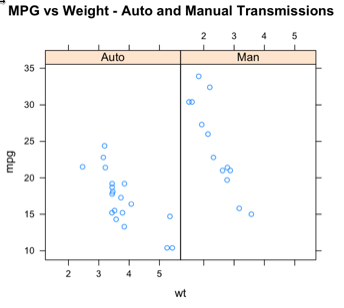
\includegraphics[height=4cm,width=4cm]{../IMG/fac1.png} & 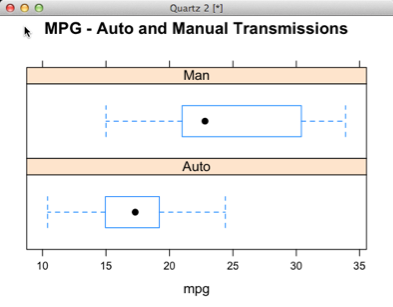
\includegraphics[height=4cm,width=4cm]{../IMG/fac2.png} \\ \hline  
\end{tabular}
\end{center}
\end{frame}


\begin{frame}[fragile]
\frametitle{Factors - aggregation preview}
With our knowledge of factors and vectors we can do some basic aggregation using the tapply command. We have a factor vector called mytransfac.
\newline
\\
Let's summarize some MPG data that corresponds to the automobiles used in the mytransfac vector. So for each car we have its MPG figure and whether it has an automatic or manual transmission.
\footnotesize
\begin{verbatim}
mympg <- c(21,21,22.8,21.4,18.7,18.1,14.3,24.4,22.8,19.2,17.8,
           16.4,17.3,15.2,10.4,10.4,14.7,32.4,30.4,33.9, 21.5,
           15.5,15.2,13.3,19.2,27.3,26,30.4,15.8,19.7,15,21.4)

# tapply( continuous_value_to_summarize,  factor_or_grouping variable,  
          function_for_summary)

tapply(mympg, mytransfac, mean)
    Auto      Man 
17.14737 24.39231 
\end{verbatim}
\end{frame}


\begin{frame}[fragile]
\frametitle{Factors - cut}
It is sometimes useful to take a continuous variable and chop it up into intervals or categories for purposes of summary or grouping. R has a function to do this called "cut" to accomplish this.
\newline
\\
Let's work through some examples to understand what is going on. Let's cut up the numbers between 0 and 10 into 4 distinct intervals
\scriptsize
\begin{verbatim}
cut(0:10,breaks=4)

[1] (-0.01,2.5] (-0.01,2.5] (-0.01,2.5] (2.5,5]   (2.5,5]  (2.5,5]  (5,7.5] 
    (5,7.5]     (7.5,10]    (7.5,10]   (7.5,10]   
Levels: (-0.01,2.5] (2.5,5] (5,7.5] (7.5,10]

table(cut(0:10,breaks=4))

(-0.01,2.5]     (2.5,5]     (5,7.5]    (7.5,10] 
          3           3           2           3 

table(cut(0:10,breaks=4))
(-0.01,2.5]     (2.5,5]     (5,7.5]    (7.5,10] 
          3           3           2           3 
\end{verbatim}
\end{frame}


\begin{frame}[fragile]
\frametitle{Factors - cut}
Well that was cool but since we are creating 4 intervals we should probably name them
\scriptsize
\begin{verbatim}
my.cut <- cut(0:10,breaks=4,labels=c("Q1","Q2","Q3","Q4")) 
[1] Q1 Q1 Q1 Q2 Q2 Q2 Q3 Q3 Q4 Q4 Q4
Levels: Q1 Q2 Q3 Q4

table(my.cut)
my.cut
Q1 Q2 Q3 Q4 
 3  3  2  3 

# But you can to take finer-grained control over how the intervals are made.

quantile(0:10)
  0%  25%  50%  75% 100% 
 0.0  2.5  5.0  7.5 10.0 

table(cut(0:10,breaks=quantile(0:10),include.lowest=TRUE))

 [0,2.5]  (2.5,5]  (5,7.5] (7.5,10] 
       3        3        2        3 

\end{verbatim}
\end{frame}


%


\begin{frame}[fragile]
\frametitle{Factors - cut}
Let's summarize some exam scores according to a typical grading system.  F: < 60, D: 60-70: C: 70-80: B:80-90 A:90-100
\scriptsize
\begin{verbatim}
set.seed(123)
exam.score <- runif(25,50,100)  # Simulate some scores

cut(exam.score,breaks=c(50,60,70,80,90,100))
 [1] (60,70]  (80,90]  (70,80]  (90,100] (90,100] (50,60]  (70,80]  (90,100]
 [9] (70,80]  (70,80]  (90,100] (70,80]  (80,90]  (70,80]  (50,60]  (90,100]
[17] (60,70]  (50,60]  (60,70]  (90,100] (90,100] (80,90]  (80,90]  (90,100]
[25] (80,90] 
Levels: (50,60] (60,70] (70,80] (80,90] (90,100]

cut(exam.score,breaks=c(50,60,70,80,90,100),labels=c("F","D","C","B","A"))
 [1] D B C A A F C A C C A C B C F A D F D A A B B A B
Levels: F D C B A

my.table <- table(cut(exam.score,breaks=c(50,60,70,80,90,100),
                  labels=c("F","D","C","B","A")))

F D C B A 
3 3 6 5 8 

barchart(my.table,main="Grade BarChart",col=terrain.colors(5))
\end{verbatim}
\end{frame}

%

\begin{frame}[fragile]
\frametitle{Factors - cut}
\begin{center}
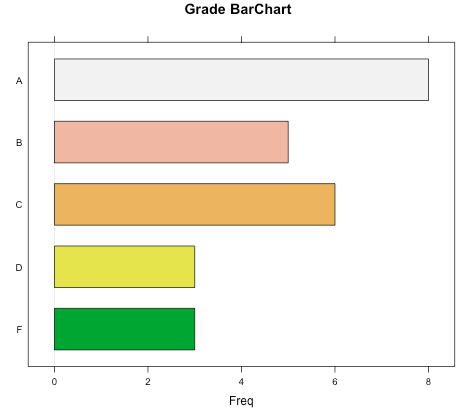
\includegraphics{../IMG/bar.png}
\end{center}
\end{frame}

%

\begin{frame}[fragile]
\frametitle{Factors - cut}
\begin{itemize}
\item But the intervals don't exactly match the grading scheme
\item A score of 90 will get a B when it should get an A
\item Note the [ and ) characters show us if the interval boundary includes a score
\item There is an argument that can help \textbf{right}) 
\end{itemize}
\scriptsize
\begin{verbatim}
set.seed(123)
cut(exam.score,breaks=c(50,60,70,80,90,100))
 [1] (60,70]  (80,90]  (70,80]  (90,100] (90,100] (50,60]  (70,80]  (90,100]
 [9] (70,80]  (70,80]  (90,100] (70,80]  (80,90]  (70,80]  (50,60]  (90,100]
[17] (60,70]  (50,60]  (60,70]  (90,100] (90,100] (80,90]  (80,90]  (90,100]
[25] (80,90] 
Levels: (50,60] (60,70] (70,80] (80,90] (90,100]

cut(exam.score,breaks=c(50,60,70,80,90,100),right=F)
 [1] [60,70)  [80,90)  [70,80)  [90,100) [90,100) [50,60)  [70,80)  [90,100)
 [9] [70,80)  [70,80)  [90,100) [70,80)  [80,90)  [70,80)  [50,60)  [90,100)
[17] [60,70)  [50,60)  [60,70)  [90,100) [90,100) [80,90)  [80,90)  [90,100)
[25] [80,90) 
Levels: [50,60) [60,70) [70,80) [80,90) [90,100)

\end{verbatim}
\end{frame}

%

\begin{frame}[fragile]
\frametitle{Factors - cut}
So if you don't think that the cut command is cool then here is how 
you would have had to solve the problem - ughhh !
\scriptsize
\begin{verbatim}
set.seed(123)
exam.score <- runif(25,50,100)

acount <- 0
bcount <- 0
ccount <- 0
dcount <- 0
fcount <- 0
exam.score <- runif(25,50,100)
for (ii in 1:length(exam.score)) {
  
 if (exam.score[ii] < 60) {fcount = fcount + 1} else
  if ((exam.score[ii] >= 60) & (exam.score[ii] < 70)) {dcount = dcount + 1} else
   if ((exam.score[ii] >= 70) & (exam.score[ii] < 80)) {ccount = ccount +1} else
    if ((exam.score[ii] >= 80) & (exam.score[ii] < 90)) {bcount = bcount +1} else
     if ((exam.score[ii] >= 90) & (exam.score[ii] <= 100)) {acount = acount +1}
}
cat("acount bcount ccount dcount fcount")
cat(acount,bcount,ccount,dcount,fcount)
acount bcount ccount dcount fcount
8 5 7 3 2

\end{verbatim}
\end{frame}

%

\begin{frame}[fragile]
\frametitle{Factors - cut}
Sometimes we want our factors to be ordered. For example, we intuitively know that January comes before February and so on. Can we get R to create ordered factors ? 
\footnotesize
\begin{verbatim}

mons <- c("Jan","Feb","Mar","Apr","May","Jun","Jan",
          "Feb","May","Jun", "Apr","Mar")

my.fact.mons <- factor(mons)
 [1] Jan Feb Mar Apr May Jun Jan Feb May Jun Apr Mar
Levels: Apr Feb Jan Jun Mar May

my.fact.mons[1] < my.fact.mons[2]

Warning message:
In Ops.factor(my.fact.mons[1], my.fact.mons[2]) :
  < not meaningful for factors

levels(my.fact.mons)
[1] "Apr" "Feb" "Jan" "Jun" "Mar" "May"
\end{verbatim}
\scriptsize
\begin{center}
\url{http://www.stat.berkeley.edu/classes/s133/factors}
\end{center}
\end{frame}


%

\begin{frame}[fragile]
\frametitle{Factors - cut}
Sometimes we want our factors to be ordered. For example, we intuitively know that January comes before February and so on. Can we get R to create ordered factors ? 
\footnotesize
\begin{verbatim}
my.fact.mons <- factor(mons, labels=c("Jan","Feb","Mar","Apr","May","Jun"),
                       ordered=TRUE)
my.fact.mons
 [1] Mar Feb May Jan Jun Apr Mar Feb Jun Apr Jan May
Levels: Jan < Feb < Mar < Apr < May < Jun

my.fact.mons[1] < my.fact.mons[2]
[1] FALSE

table(my.fact.mons)
my.fact.mons
Jan Feb Mar Apr May Jun 
  2   2   2   2   2   2 

levels(my.fact.mons)                       # This is what we want !
[1] "Jan" "Feb" "Mar" "Apr" "May" "Jun"
\end{verbatim}
\scriptsize
\begin{center}
\url{http://www.stat.berkeley.edu/classes/s133/factors}
\end{center}
\end{frame}


%

\begin{frame}[fragile]
\frametitle{Factors - cut}
Let's do an AOV on the mtcars data set variables MPG and number of gears the latter of which takes on the values 3,4,5. So it is well suited to be a factor.
\scriptsize
\begin{verbatim}
mtcars$gear <- factor(mtcars$gear)  # Turn gear into a factor
aov.ex1 = aov(mpg ~ gear,mtcars)
summary(aov.ex1)
             Df Sum Sq Mean Sq F value    Pr(>F)    
factor(gear)  2 483.24 241.622  10.901 0.0002948 ***
Residuals    29 642.80  22.166                      
---
Signif. codes:  0 '***' 0.001 '**' 0.01 '*' 0.05 '.' 0.1 ' ' 1 
print(model.tables(aov.ex1,"means"))
Tables of means
Grand mean
         
20.09062 

 gear 
        3     4     5
    16.11 24.53 21.38
rep 15.00 12.00  5.00

\end{verbatim}
\scriptsize
\end{frame}

\begin{frame}[fragile]
\frametitle{Factors - cut}
Let's do an AOV on the mtcars data set variables MPG and number of gears the latter of which takes on the values 3,4,5. So it is well suited to be a factor.
\scriptsize
\begin{verbatim}
 
my.tukey <- TukeyHSD(aov.ex1,"gear")  # Tukey Multiple Comparisons
my.tukey
  Tukey multiple comparisons of means
    95% family-wise confidence level

Fit: aov(formula = mpg ~ gear, data = mtcars)

$gear
         diff        lwr       upr     p adj
4-3  8.426667  3.9234704 12.929863 0.0002088
5-3  5.273333 -0.7309284 11.277595 0.0937176
5-4 -3.153333 -9.3423846  3.035718 0.4295874

plot(my.tukey)
\end{verbatim}
\normalsize
Differences between Gears are significant at the five percent level if the confidence interval around 
the estimation of the difference does not contain zero
\scriptsize
\end{frame}

%


\begin{frame}[fragile]
\frametitle{Factors - cut}
\begin{center}
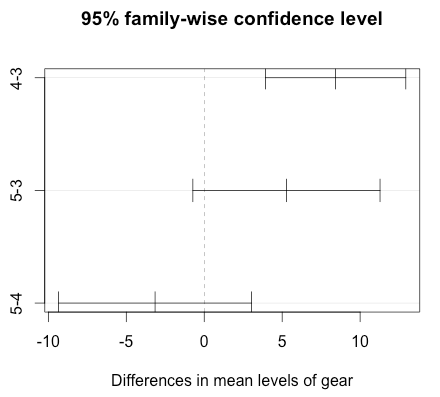
\includegraphics{../IMG/tukey.png}
\end{center}
\end{frame}
%%%

\section{Matrices}
\begin{frame}[fragile]
\frametitle{Matrices}
\begin{itemize}

\item Matrices are important mathematical structures for which R has excellent support
\vspace{0.15cm}
\item Matrices are ideal for storing information on scientific data
\vspace{0.15cm}
\item Think of a matrix as being a vector with dimnensions
\vspace{0.15cm}
\item There are two common ways to create a matrix

\end{itemize}

\end{frame}


\begin{frame}[fragile]
\frametitle{Matrices - Creating}
1) Using the \textbf{dim()} function. You can think of the following vector as being a matrix with one row and twelve columns. 
\footnotesize
\begin{verbatim}
myvec <- c(1:12)
\end{verbatim}
\normalsize
To create, for example, a 3x4 matrix use the \textbf{dim()} function to adjust the dimensions of the vector
\footnotesize
\begin{verbatim}
dim(myvec) <- c(3,4)
myvec
     [,1] [,2] [,3] [,4]
[1,]    1    4    7   10
[2,]    2    5    8   11
[3,]    3    6    9   12
\end{verbatim}
\normalsize
Note that columns are "filled" before rows. Note also that the requested dimension must make sense with the available number of elements
\footnotesize
\begin{verbatim}
dim(myvec <- c(5,4))
Error in dim(myvec = c(5, 4)) : 
supplied argument name 'myvec' does not match 'x'
\end{verbatim}
\end{frame}

\begin{frame}[fragile]
\frametitle{Matrices - Creating}
2) Using the \textbf{matrix()} function. 
\footnotesize
\begin{verbatim}
mymat <- matrix( c(7, 4, 2, 4, 7, 2), nrow=3, ncol=2) 
     [,1] [,2]
[1,]    7    4
[2,]    4    7
[3,]    2    2
\end{verbatim}
\normalsize
\vspace{0.25cm}
You can use the \textbf{nrow} and \textbf{ncol} arguments to explicity specify the desired number of rows and columns. You can also request that the rows get filled first as opposed to the columns:
\footnotesize
\begin{verbatim}
mymat <- matrix( c(7, 4, 2, 4, 7, 2), nrow=3, ncol=2, byrow=TRUE)
mymat
     [,1] [,2]
[1,]    7    4
[2,]    2    4
[3,]    7    2
\end{verbatim}
\normalsize
\end{frame}


\begin{frame}[fragile]
\frametitle{Matrices - Naming Rows and Columns}
It is useful to name the rows and columns of matrices
\footnotesize
\begin{verbatim}
set.seed(123)
X <- matrix(rpois(20,1.5),nrow=4)
X
     [,1] [,2] [,3] [,4] [,5]
[1,]    1    4    1    2    1
[2,]    2    0    1    2    0
[3,]    1    1    4    0    1
[4,]    3    3    1    3    4
\end{verbatim}
\normalsize
\vspace{0.25cm}
Let's say that these refer to four trials. We want to label the rows "Trial.1", "Trial.2", etc.
\footnotesize
\begin{verbatim}
rownames(X) <- paste("Trial",1:nrow(X),sep=".")
X
        [,1] [,2] [,3] [,4] [,5]
Trial.1    1    4    1    2    1
Trial.2    2    0    1    2    0
Trial.3    1    1    4    0    1
Trial.4    3    3    1    3    4
\end{verbatim}
\end{frame}


\begin{frame}[fragile]
\frametitle{Matrices - Naming Rows and Columns}
We can something similar with the columns
\small
\begin{verbatim}
colnames(X) <- paste("P",1:ncol(X),sep=".")
 
X
        P.1 P.2 P.3 P.4 P.5
Trial.1   1   4   1   2   1
Trial.2   2   0   1   2   0
Trial.3   1   1   4   0   1
Trial.4   3   3   1   3   4
\end{verbatim}
\scriptsize
Example taken from ``The R Book - Michael J. Crawley
\end{frame}


\begin{frame}[fragile]
\frametitle{Matrices - Naming Rows and Columns}
We aren't restricted to naming things according to a pattern
\footnotesize
\begin{verbatim}
drug.names <- c("aspirin","paracetamol","nurofen","hedex","placebo")

colnames(X) <- drug.names

X
        aspirin paracetamol nurofen hedex placebo
Trial.1       1           4       1     2       1
Trial.2       2           0       1     2       0
Trial.3       1           1       4     0       1
Trial.4       3           3       1     3       4

\end{verbatim}
\scriptsize
Example taken from ``The R Book - Michael J. Crawley
\end{frame}


\begin{frame}[fragile]
\frametitle{Matrices - Indexing}
Names provide an intutive way to index into a matrix structure
\footnotesize
\begin{verbatim}
X
        aspirin paracetamol nurofen hedex placebo
Trial.1       1           4       1     2       1
Trial.2       2           0       1     2       0
Trial.3       1           1       4     0       1
Trial.4       3           3       1     3       4

X['Trial.1',]   # Gets all columns for Trial #1

    aspirin paracetamol     nurofen       hedex     placebo 
          1           4           1           2           1 

# Get's the nurofen column for Trial.1

X['Trial.1','nurofen']
[1] 1
\end{verbatim}
\scriptsize
Example taken from ``The R Book - Michael J. Crawley
\end{frame}


\begin{frame}[fragile]
\frametitle{Matrices - Indexing}
Names provide an intutive way to index into a matrix structure
\footnotesize
\begin{verbatim}
X
        aspirin paracetamol nurofen hedex placebo
Trial.1       1           4       1     2       1
Trial.2       2           0       1     2       0
Trial.3       1           1       4     0       1
Trial.4       3           3       1     3       4


X[,'nurofen']                     # Get all Trials for nurofen
Trial.1 Trial.2 Trial.3 Trial.4 
      1       1       4       1 

X[,'nurofen',drop=FALSE]   # Preserves matrix structure if desired
  nurofen
Trial.1       1
Trial.2       1
Trial.3       4
Trial.4       1

\end{verbatim}
\scriptsize
Example taken from ``The R Book - Michael J. Crawley
\end{frame}

\begin{frame}[fragile]
\frametitle{Matrices - Indexing}
It is more common to use numeric indexing especially if you are accessing parts of a matrix from a program
\scriptsize
\begin{verbatim}
set.seed(123)
X <- matrix(rpois(9,1.5),nrow=3)
X
     [,1] [,2] [,3]
[1,]    1    3    1
[2,]    2    4    3
[3,]    1    0    1

X[1,1]     # First row, First Column
[1] 1

X[2,2]     # Second row, Second Column
[1] 4

X[3,3]     # Third row, Third column
1] 1

diag(X)     # Ah, there is a function that gets the diagonal.
[1] 1 4 1   # Always check to see if there is already a function
            # to do what you want
\end{verbatim}
\scriptsize
Example taken from ``The R Book - Michael J. Crawley
\end{frame}


\begin{frame}[fragile]
\frametitle{Matrices - Indexing}
Extracting information from a matrix is an important skill. Practice makes perfect
\scriptsize
\begin{verbatim}
X
     [,1] [,2] [,3]
[1,]    1    3    1
[2,]    2    4    3
[3,]    1    0    1


X[1:2,1]     # Gets First and second rows and the first column
[1] 1 2

X[1:2,2]     # Gets First and second rows and the second column
[1] 3 4

X[1:2,]      # Gets First and second rows and ALL columns
    [,1] [,2] [,3]
[1,]    1    3    1
[2,]    2    4    3

\end{verbatim}
\scriptsize
Example taken from ``The R Book - Michael J. Crawley
\end{frame}

\begin{frame}[fragile]
\frametitle{Matrices - Indexing}
Extracting information from a matrix is an important skill. Practice makes perfect
\scriptsize
\begin{verbatim}
X
     [,1] [,2] [,3]
[1,]    1    3    1
[2,]    2    4    3
[3,]    1    0    1

X[,c(1,3)]     # Get all rows but only columns 1 and 3
      [,1] [,2]
[1,]    1    1
[2,]    2    3
[3,]    1    1


X[,-2]   # Same effect as above. Get all rows and columns except 2
     [,1] [,2]
[1,]    1    1
[2,]    2    3
[3,]    1    1
\end{verbatim}
\scriptsize
Example taken from ``The R Book - Michael J. Crawley
\end{frame}


\begin{frame}[fragile]
\frametitle{Matrices - Indexing}
Remember that a matrix is just a vector with dimensions so you could index into a matrix using single bracket notation.
\scriptsize
\begin{verbatim}
X
     [,1] [,2] [,3]
[1,]    1    3    1
[2,]    2    4    3
[3,]    1    0    1

X[1:4]
[1] 1 2 1 3

X >= 2
      [,1]  [,2]  [,3]
[1,] FALSE  TRUE FALSE
[2,]  TRUE  TRUE  TRUE
[3,] FALSE FALSE FALSE


X[X >= 2]   # Returns which values are greater or equal to 2
[1] 2 3 4 3

which(X >= 2)   # Returns which elements are greater or equal to 2
[1] 2 4 5 8
\end{verbatim}
\end{frame}

\begin{frame}[fragile]
\frametitle{Matrices - Indexing}
Remember that a matrix is just a vector with dimensions so you could index into a matrix using single bracket notation.
\footnotesize
\begin{verbatim}

     [,1] [,2] [,3]
[1,]    1    3    1
[2,]    2    4    3
[3,]    1    0    1

X %% 2 == 0          # Returns a logical matrix
      [,1]  [,2]  [,3]
[1,] FALSE FALSE FALSE
[2,]  TRUE  TRUE FALSE
[3,] FALSE  TRUE FALSE


X[ X %% 2 == 0 ]   # Finds the actual element values
[1] 2 4 0


\end{verbatim}
\end{frame}

%

\begin{frame}[fragile]
\frametitle{Matrices - Indexing}
Remember that a matrix is just a vector with dimensions so you could index into a matrix using single bracket notation.
\footnotesize
\begin{verbatim}
X
     [,1] [,2] [,3]
[1,]    1    3    1
[2,]    2    4    3
[3,]    1    0    1


X[X %%  2 == 0] <- 99

X
     [,1] [,2] [,3]
[1,]    1    3    1
[2,]    99   99   3
[3,]    1    99   1
\end{verbatim}
\end{frame}

%

\begin{frame}[fragile]
\frametitle{Matrices - Indexing}
There are two functions called row and col that return the numeric row and column, respectively of the matrix. 
\footnotesize
\begin{verbatim}
X
     [,1] [,2] [,3]
[1,]    1    3    1
[2,]    2    4    3
[3,]    1    0    1

row(X)
     [,1] [,2] [,3]
[1,]    1    1    1   # The values correspond to the actual row number
[2,]    2    2    2
[3,]    3    3    3

col(X)                # The values correspond to the actual col number
     [,1] [,2] [,3]
[1,]    1    2    3
[2,]    1    2    3
[3,]    1    2    3
\end{verbatim}
\end{frame}

%

\begin{frame}[fragile]
\frametitle{Matrices - Indexing}
There are two functions called row and col that return the numeric row and column, respectively of the matrix. 
\footnotesize
\begin{verbatim}
row(X) == col(X)

      [,1]  [,2]  [,3]
[1,]  TRUE FALSE FALSE
[2,] FALSE  TRUE FALSE
[3,] FALSE FALSE  TRUE
 

X[row(X) == col(X)]
[1] 1 4 1

X[row(X) == col(X)] <- 0  # Put zeroes in the diagonal

     [,1] [,2] [,3]
[1,]    0    3    1
[2,]    2    0    3
[3,]    1    0    0

\end{verbatim}
\end{frame}

%

\begin{frame}[fragile]
\frametitle{Matrices - rbind/cbind}
Sometimes we need to add rows and columns to a matrix. There are two commands to do this: rbind and cbind. 
\footnotesize
\begin{verbatim}
set.seed(123) 

X <- matrix(rpois(9,1.5),nrow=3)

colnames(X) <- c("aspirin","paracetamol","nurofen")

rownames(X) <- paste("Trial",1:3,sep=".")

 
rbind(X,Trial.4=c(4,7,5))
        aspirin paracetamol nurofen
Trial.1       1           3       1
Trial.2       2           4       3
Trial.3       1           0       1
Trial.4       4           7       5

\end{verbatim}
\end{frame}

%

\begin{frame}[fragile]
\frametitle{Matrices - rbind/cbind}
Binding columns works pretty much the same way:
\footnotesize
\begin{verbatim}

X
        aspirin paracetamol nurofen
Trial.1       1           3       1
Trial.2       2           4       3
Trial.3       1           0       1


rowSums(X)
Trial.1 Trial.2 Trial.3 
      5       9       2 

cbind(X,rowsums = rowSums(X))
        aspirin paracetamol nurofen rowsums
Trial.1       1           3       1       5
Trial.2       2           4       3       9
Trial.3       1           0       1       2

\end{verbatim}
\end{frame}

%

\begin{frame}[fragile]
\frametitle{Matrices - Calculations}
Let's look at some examples involving calculations on matricies:
\footnotesize
\begin{verbatim}
set.seed(123) 

X <- matrix(rpois(9,1.5),nrow=3)

colnames(X) <- c("aspirin","paracetamol","nurofen")

rownames(X) <- paste("Trial",1:3,sep=".")

X
        aspirin paracetamol nurofen
Trial.1       1           3       1
Trial.2       2           4       3
Trial.3       1           0       1

mean(X[,3])  # Mean of the 3rd column
[1] 1.666667

var(X[3,]) # Variance of the 3rd row
[1] 0.3333333
\end{verbatim}
\end{frame}


%

\begin{frame}[fragile]
\frametitle{Matrices - Calculations}
There are functions optimized specifcally for use with matrices. They are very fast and work well on large matrices
\footnotesize
\begin{verbatim}
X
        aspirin paracetamol nurofen
Trial.1       1           3       1
Trial.2       2           4       3
Trial.3       1           0       1

rowSums(X)
Trial.1 Trial.2 Trial.3 
      5       9       2 

colSums(X)
aspirin paracetamol     nurofen 
   4           7           5 
\end{verbatim}
\end{frame}

%

\begin{frame}[fragile]
\frametitle{Matrices - Calculations}
There are functions optimized specifcally for use with matrices. They are very fast and work well on large matrices. \\
\vspace{0.25cm}
However be careful if the matrix has missing data in wich case you will need to include the \textbf{na.rm=TRUE} arugement.
\footnotesize
\begin{verbatim}
rowMeans(X)
  Trial.1   Trial.2   Trial.3 
1.6666667 3.0000000 0.6666667 

colMeans(X,na.rm=TRUE)
    aspirin paracetamol     nurofen 
   1.333333    2.333333    1.666667 
 
colMeans(X)[3]
 nurofen 
1.666667 
\end{verbatim}
\end{frame}

%

\begin{frame}[fragile]
\frametitle{Matrices - Calculations}
There are functions optimized specifcally for use with matrices. They are very fast and work well on large matrices. \\
\vspace{0.25cm}
However be careful if the matrix has missing data in wich case you will need to include the \textbf{na.rm=TRUE} arugement.
\footnotesize
\begin{verbatim}
X[1,2] <- NA
X
        aspirin paracetamol nurofen
Trial.1       1          NA       1
Trial.2       2           4       3
Trial.3       1           0       1


colMeans(X)
    aspirin paracetamol     nurofen 
   1.333333          NA    1.666667 
 
colMeans(X, na.rm=TRUE)
    aspirin paracetamol     nurofen 
   1.333333    2.000000    1.666667 

\end{verbatim}
\end{frame}

%

\begin{frame}[fragile]
\frametitle{Matrices - apply}
There is a function called \textbf{apply} which simplifies looping over the rows or columns of a matrix. The ``apply family'' of functions is important in R.
\footnotesize
\begin{verbatim}
X
        aspirin paracetamol nurofen
Trial.1       3           1       3
Trial.2       2           2       2
Trial.3       2           0       5

apply(X,1,range)            # 1 is for rows
     Trial.1 Trial.2 Trial.3
[1,]       1       2       0
[2,]       3       4       1

apply(X,2,range)            # 2 is for columns
     aspirin paracetamol nurofen
[1,]       1           0       1
[2,]       2           4       3
\end{verbatim}
\end{frame}

%

\begin{frame}[fragile]
\frametitle{Matrices - Linear Algebra}
R supports common linear algebra operations
\footnotesize
\begin{equation}
A = \begin{bmatrix}
       1 & 2 \\[0.3em]
       3 & 8 \\[0.3em]
       2 & 9 \\
     \end{bmatrix}
t(A) = \begin{bmatrix}
        1 & 3 & 2 \\[0.3em]
        2 & 8 & 9 \\[0.3em]
       \end{bmatrix}
\end{equation}
\footnotesize
\begin{verbatim}
A = matrix(c(1,3,2,2,8,9),3,2)
A
     [,1] [,2]
[1,]    1    2
[2,]    3    8
[3,]    2    9


t(A)
     [,1] [,2] [,3]
[1,]    1    3    2
[2,]    2    8    9

\end{verbatim}
\end{frame}


%

\begin{frame}[fragile]
\frametitle{Matrices - Linear Algebra}
\scriptsize
\begin{verbatim}
B
     [,1] [,2]
[1,]    5    4
[2,]    8    2

diag(B)             # Fetches the diagonal
[1] 5 2

diag(c(1,2,3))      # Creates a matrix with 1,2,3 on the diagonal
     [,1] [,2] [,3]
[1,]    1    0    0
[2,]    0    2    0
[3,]    0    0    3

diag(1,4)           # Creates a 4 x 4 Indentity matrix
     [,1] [,2] [,3] [,4]
[1,]    1    0    0    0
[2,]    0    1    0    0
[3,]    0    0    1    0
[4,]    0    0    0    1
\end{verbatim}
\end{frame}

%

\begin{frame}[fragile]
\frametitle{Matrices - Linear Algebra}
The inverse of a n x n matrix A is the matrix B (which is also n x n) that when multiplied by A gives the identity matrix
\footnotesize
\begin{verbatim}
A <- matrix(1:4,2,2)
A
     [,1] [,2]
[1,]    1    3
[2,]    2    4

B = solve(A)

B
     [,1] [,2]
[1,]   -2  1.5
[2,]    1 -0.5

A %*% B            # We get the identity matrix
     [,1] [,2]
[1,]    1    0
[2,]    0    1
\end{verbatim}
\scriptsize
\url{http://bendixcarstensen.com/APC/linalg-notes-BxC.pdf}
\end{frame}

%

\begin{frame}[fragile]
\frametitle{Matrices - Linear Algebra}
Suppose we have the following system of equations
\begin{tabular}{| l | l |}
  \hline         
  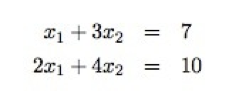
\includegraphics[height=1.5cm,width=4cm]{../IMG/eqn1.png} & 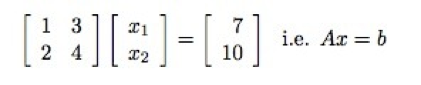
\includegraphics[height=1.5cm,width=6cm]{../IMG/eq2.png} \\ \hline  
\end{tabular}

\footnotesize
\begin{verbatim}
A
     [,1] [,2]
[1,]    1    3
[2,]    2    4

b = c(7,10)
x = solve(A) %*% b
x
     [,1]
[1,]    1
[2,]    2
\end{verbatim}
\scriptsize
\url{http://bendixcarstensen.com/APC/linalg-notes-BxC.pdf}
\end{frame}

%

\begin{frame}[fragile]
\frametitle{Matrices - Eigen values}
Eigen values/vectors show up a lot in math - like with Principal Components
\scriptsize
\begin{verbatim}
my.wines <- read.csv("http://steviep42.bitbucket.org/YOUTUBE.DIR/wines.csv",
                      header=T)
my.scaled.wines <- scale(my.wines[,-1])   # Scale the data
my.cov <- cor(my.wines[,-1])       # Get the covariance matrix
my.eigen <- eigen(my.cov)            # Now find the eigen values/vectors

options(digits=3)                 
my.eigen                            # Check out the Eigen values and vectors
$values
[1]  4.76e+00  1.81e+00  3.53e-01  7.44e-02  3.73e-16 -2.61e-16 -2.99e-16

$vectors
        [,1]    [,2]     [,3]    [,4]      [,5]      [,6]      [,7]
[1,] -0.3965  0.1149  0.80247  0.0519 -1.46e-01  0.00e+00 -4.02e-01
[2,] -0.4454 -0.1090 -0.28106 -0.2745  4.84e-01 -5.18e-01 -3.64e-01
[3,] -0.2646 -0.5854 -0.09607  0.7603  5.41e-16  3.75e-16 -1.16e-15
[4,]  0.4160 -0.3111  0.00734 -0.0939  3.24e-01  4.88e-01 -6.15e-01
[5,] -0.0485 -0.7245  0.21611 -0.5474 -2.16e-01 -3.23e-02  2.80e-01
[6,] -0.4385  0.0555 -0.46576 -0.1687 -5.67e-01  3.86e-01 -2.97e-01
[7,] -0.4547  0.0865  0.06430 -0.0835  5.20e-01  5.85e-01  4.01e-01

$loadings <- my.eigen$vectors
\end{verbatim}
\scriptsize
\url{http://bendixcarstensen.com/APC/linalg-notes-BxC.pdf}
\end{frame}

%

\begin{frame}[fragile]
\frametitle{Matrices - Eigen values}
Eigen values/vectors show up a lot in math - like with Principal Components. The loadings dervied in the previous slide are the principal componenents
\newline

\begin{verbatim}
loadings <- my.eigen$vectors
\end{verbatim}
\normalsize
The scores are the product of the matrix multiplication between the scaled.wines and the loadings. This takes the original wine data and re-expresses it in terms of the "principal components".  
\begin{verbatim}
scores <- my.scaled.wines %*% loadings 
\end{verbatim}

\end{frame}

%

\begin{frame}[fragile]
\frametitle{Matrices - Clustering}
Matrices are also used a lot in cluster analysis. Let's look at a matrix of 32 cars and attempt to cluster them according to their various attributes such as MPG, Number of Cylinders, Gears, Weight, etc. This data set (mtcars) is internal to R so you can refer to it easily.
\newline
\scriptsize
\begin{verbatim}
                    mpg cyl  disp  hp drat   wt qsec vs am gear carb
Mazda RX4           21.0   6 160.0 110 3.90 2.62 16.5  0  1    4    4
Mazda RX4 Wag       21.0   6 160.0 110 3.90 2.88 17.0  0  1    4    4
Datsun 710          22.8   4 108.0  93 3.85 2.32 18.6  1  1    4    1
Hornet 4 Drive      21.4   6 258.0 110 3.08 3.21 19.4  1  0    3    1
Hornet Sportabout   18.7   8 360.0 175 3.15 3.44 17.0  0  0    3    2
..
..

# We first compute a distance between the rows and then cluster them.

hc <- hclust(dist(mtcars[,2:11]))  # The first column is a label. 
plot(hc, hang = -1,cex=0.7)

\end{verbatim}
\end{frame}

%

\begin{frame}[fragile]
\frametitle{Matrices - Eigen values}
\begin{center}
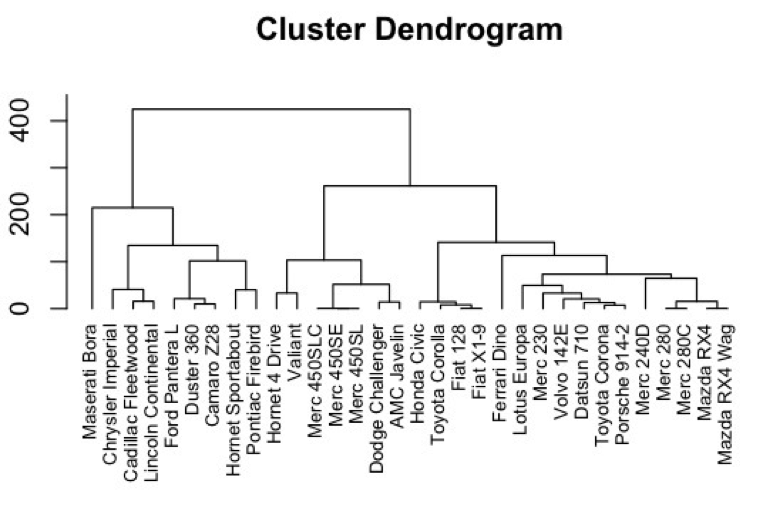
\includegraphics{../IMG/dendro.png}
\end{center}
\end{frame}


%

\begin{frame}[fragile]
\frametitle{Matrices - replicate}
\begin{itemize}
\item We can create matrices using the replicate command
\item Useful when doing repeated sampling activity like bootstrapping
\end{itemize}
\footnotesize
\begin{verbatim}
replicate(4,rnorm(5))
             [,1]       [,2]       [,3]        [,4]
[1,] -1.181720384  0.2717525 -1.4716542  2.26654104
[2,]  0.268970133  0.3423814  0.9553185  0.07749788
[3,]  0.007413904 -1.2102476  0.2273662 -0.46742459
[4,]  1.726961040  0.9977138  2.0491924  0.77174367
[5,]  0.950821481 -1.8599874 -0.8587209  0.95906263

some.population <- rnorm(1000)

replicate(4,sample(some.population, 5, replace=TRUE))
           [,1]        [,2]       [,3]       [,4]
[1,] -0.4680211  0.27727612 -0.5346220 0.94161600
[2,]  0.3138391  0.36105532  0.1108916 0.35186402
[3,] -1.8416441 -0.05812402  1.3535505 0.05288187
[4,] -0.9483933 -0.24572418  1.6950778 1.30636068
[5,]  1.0369327 -0.66983941  0.3055545 1.57318148
\end{verbatim}
\end{frame}

%

\begin{frame}[fragile]
\frametitle{Matrices - Functions}
\begin{center}
\footnotesize
\begin{tabular}{| l | l |}
  \hline     
  \textbf{Operation} & \textbf{Description} \\ \hline
  A * B & Element-wise multiplication \\ \hline
  A %*% B & Matrix multiplication \\ \hline
  t(A) & Transpose \\ \hline
  diag(x) & Creates diagonal matrix with elements of x in diagonal \\ \hline
  diag(A) & Returns a vector with the elements of the diagonal \\ \hline
  diag(k) & Creates a k x k identity matrix \\ \hline
  solve(A,b) & Returns vector x in the equation b = Ax \\ \hline
  solve(A) & Inverse of A where A is a square matrix \\ \hline
  y <- eigen(A) & Gets eigenvalues and eigenvectors of A \\ \hline
  y <- svd(A) & Single value decomposition of A \\ \hline
  y <- qr(A) & QR decomposition of A \\ \hline
  cbind(A,B,...) & Combine matrices/vectors horizontally \\ \hline
  rbind(A,B,...) & Combine matrices/vectors vertically \\ \hline
  rowMeans(A) & Retruns vector of row means \\ \hline
  rowSums(A) & Returns vector of row sums \\ \hline
  colMeans(A) & Returns vector of column means \\ \hline
  colSums(A) & Returns vector of column means \\ \hline
\end{tabular}
\end{center}
\end{frame}

\section{Lists}
%% Lists


%
\begin{frame}[fragile]
\frametitle{Lists}
\begin{itemize}
\item Lists provide a way to store information of different 
   types within a single data structure 
\item Remember that vectors and matrices restrict us to only one data type at a time. 
\item That is we cannot mix, for example, characters and numbers within a vector or matrix. 
\item Many functions in R return information stored in lists
\item Consider the following example wherein we store information about a family. Not all this 
information is of the same type
\end{itemize}
\end{frame}

%
\begin{frame}[fragile]
\frametitle{Lists}
\scriptsize
\begin{verbatim}
family1 <- list(husband="Fred", wife="Wilma", numofchildren=3, 
                agesofkids=c(8,11,14))

length(family1)  # Has 4 elements
[1] 4

family1
$husband
[1] "Fred"

$wife
[1] "Wilma"

$numofchildren
[1] 3

$agesofkids
[1]  8 11 14

str(family1)
List of 4
 $ husband      : chr "Fred"
 $ wife         : chr "Wilma"
 $ numofchildren: num 3
 $ agesofkids   : num [1:3] 8 11 14
\end{verbatim}

\end{frame}

%
%
\begin{frame}[fragile]
\frametitle{Lists - Creating}
If possible, always create named elements. It is easier for humans to index into a named list
\scriptsize
\begin{verbatim}
family1 <- list(husband="Fred", wife="Wilma", numofchildren=3, 
                agesofkids=c(8,11,14))
                
# If the list elements have names then use "$" to access the element

family1$agesofkids   
[1]  8 11 14

family1$agesofkids[1:2]
[1]  8 11

# Checkout the sapply command 

sapply(family1,class)
      husband          wife numofchildren    agesofkids 
  "character"   "character"     "numeric"     "numeric" 

sapply(family1,length)
      husband          wife numofchildren    agesofkids 
            1             1             1             3 
\end{verbatim}
\end{frame}

%
\begin{frame}[fragile]
\frametitle{Lists - Creating}
If the list elements have no names then you have to use numeric indexing
\footnotesize
\begin{verbatim}
family2 <- list("Barney","Betty",2,c(4,6))
[[1]]
[1] "Barney"

[[2]]
[1] "Betty"

[[3]]
[1] 2

[[4]]
[1] 4 6

\end{verbatim}
\end{frame}


%
\begin{frame}[fragile]
\frametitle{Lists - Creating}
If the list elements have no names then you have to use numeric indexing
\footnotesize
\begin{verbatim}
family2 <- list("Barney","Betty",2,c(4,6))

family2[4]    # Accesses the 4th index and associated element 
[[1]]
[1] 4 6

family2[[4]]   # Accesses the 4th element value only - more direct
[1] 4 6

family2[3:4]   # Get 3rd and 4th indices and associate values
[[1]]
[1] 2

[[2]]
[1] 4 6

\end{verbatim}
\end{frame}

%
\begin{frame}[fragile]
\frametitle{Lists - unlist()}
Use the ``unlist'' function to turn a list into a vector. Since the list usually has mixed data types then the elements will be converted to a single type.
\footnotesize
\begin{verbatim}
family1 <- list(husband="Fred", wife="Wilma", numofchildren=3, 
                agesofkids=c(8,11,14))
                
unlist(family1)
husband   wife  numofchildren   agesofkids1   agesofkids2   agesofkids3 
 "Fred" "Wilma"       "3"           "8"          "11"          "14" 

as.numeric(unlist(family1))
[1] NA NA  3  8 11 14

\end{verbatim}
\end{frame}

%
\begin{frame}[fragile]
\frametitle{Lists - Uses}
As newcomers to R we usually doesn't create lists except in two major cases:
\begin{itemize}

\item We are writing a function that does some interesting stuff and we want to return to the user
a structure that has information of varying types

\item As a precursor to creating a a data frame, which represents a hybrid object with characteristics of a list and a matrix
\end{itemize}
\footnotesize
\end{frame}

%
\begin{frame}[fragile]
\frametitle{Lists - Functions}
As an example of the first case, R has lots of statistical functions that return lists of information.
\small
\begin{verbatim}
data(mtcars)   # Load mtcars into the environment

mylm <- lm(mpg ~ wt, data = mtcars)

print(mylm)

Call:
lm(formula = mpg ~ wt, data = mtcars)

Coefficients:
(Intercept)           wt  
     37.285       -5.344  

# But there is a lot more information

typeof(mylm)
[1] "list"
\end{verbatim}
\end{frame}

%
\begin{frame}[fragile]
\frametitle{Lists - Functions}

\scriptsize
\begin{verbatim}
str(mylm,give.attr=F)  # Lots of stuff here

List of 12
 $ coefficients : Named num [1:2] 37.29 -5.34
 $ residuals    : Named num [1:32] -2.28 -0.92 -2.09 1.3 -0.2 ...
 $ effects      : Named num [1:32] -113.65 -29.116 -1.661 1.631 0.111 ...
 $ rank         : int 2
 $ fitted.values: Named num [1:32] 23.3 21.9 24.9 20.1 18.9 ...
 $ assign       : int [1:2] 0 1
 $ qr           :List of 5
  ..$ qr   : num [1:32, 1:2] -5.657 0.177 0.177 0.177 0.177 ...
  ..$ qraux: num [1:2] 1.18 1.05
  ..$ pivot: int [1:2] 1 2
  ..$ tol  : num 1e-07
  ..$ rank : int 2
 $ df.residual  : int 30
 $ xlevels      : Named list()
 $ call         : language lm(formula = mpg ~ wt, data = mtcars)
 $ terms        :Classes 'terms', 'formula' length 3 mpg ~ wt
 $ model        :'data.frame':  32 obs. of  2 variables:
  ..$ mpg: num [1:32] 21 21 22.8 21.4 18.7 18.1 14.3 24.4 22.8 19.2 ...
  ..$ wt : num [1:32] 2.62 2.88 2.32 3.21 3.44 ...

\end{verbatim}
\end{frame}

%
\begin{frame}[fragile]
\frametitle{Lists - Functions}
\scriptsize
\begin{verbatim}
names(mylm)
 [1] "coefficients"  "residuals"     "effects"       "rank"         
 [5] "fitted.values" "assign"        "qr"            "df.residual"  
 [9] "xlevels"       "call"          "terms"         "model"  

mylm$effects
 (Intercept)           wt                                                     
-113.6497374  -29.1157217   -1.6613339    1.6313943    0.1111305   -0.3840041                                                                             
  -3.6072442    4.5003125    2.6905817    0.6111305   -0.7888695    1.1143917                                                                              
   0.2316793   -1.6061571    1.3014525    2.2137818    6.0995633    7.3094734                                                                               
   2.2421594    6.8956792   -2.2010595   -2.6694078   -3.4150859   -3.1915608                                                                               
   2.7346556    0.8200064    0.5948771    1.7073457   -4.2045529   -2.4018616                           
  -2.9072442   -0.6494289 

# Some use the $ notation to extract desired information they want straight 
# from the function call

lm(mpg ~ wt, data = mtcars)$coefficients
(Intercept)          wt 
  37.285126   -5.344472 

\end{verbatim}
\end{frame}

%
\begin{frame}[fragile]
\frametitle{Lists - Functions}
Some other basic R functions will return a list - such as some of the character functions:
\scriptsize
\begin{verbatim}
mystring <- "This is a test"

mys <- strsplit(mystring, " ")

str(mys)
List of 1
 $ : chr [1:4] "This" "is" "a" "test"

mys
[[1]]
[1] "This" "is"   "a"    "test"

mys[[1]][1]
[1] "This" 

mys[[1]][1:2]
[1] "This" "is"  

unlist(mys)
[1] "This" "is"   "a"    "test"
\end{verbatim}
\end{frame}
%
\begin{frame}[fragile]
\frametitle{Lists - Functions}
When we create our own functions we can return a list
\scriptsize
\begin{verbatim}
my.summary <- function(x) {
  return.list <- list()      
  return.list$mean <- mean(x)
  return.list$sd <- sd(x)
  return.list$var <- var(x)
  return(return.list)   
}

my.summary(1:10)
$mean
[1] 5.5

$sd
[1] 3.02765

$var
[1] 9.166667

names(my.summary(1:10))
[1] "mean" "sd"   "var" 

my.summary(1:10)$var     
[1] 9.166667
\end{verbatim}
\end{frame}

%
\begin{frame}[fragile]
\frametitle{Lists - sapply/lapply}
Remember the sapply command ? We use it to apply a function over each element of a list or a vector. This helps us avoid having to write a ``for-loop'' every time we want to process a list or a vector.
\footnotesize
\begin{verbatim}
# sapply( vector_or_list, function_to_apply_to_each element)

family1 <- list(husband="Fred", wife="Wilma", numofchildren=3, 
                agesofkids=c(8,11,14))

sapply(family1,class)
      husband          wife numofchildren    agesofkids 
  "character"   "character"     "numeric"     "numeric" 

sapply(family1,length)
      husband          wife numofchildren    agesofkids 
            1             1             1             3 

\end{verbatim}
\end{frame}

%

%
\begin{frame}[fragile]
\frametitle{Lists - sapply/lapply}
\textbf{sapply} tries to return a "simplified" version of the output (either a vector or matrix) hence the "s" in the "sapply". If you don't use something like sapply then the example on the previous slide would look this:
\footnotesize
\begin{verbatim}

# sapply( vector_or_list, function_to_apply_to_each element)

family1 <- list(husband="Fred", wife="Wilma", numofchildren=3, 
                agesofkids=c(8,11,14))

for (ii in 1:length(family1)) {
   cat(names(family1)[ii]," : ",class(family1[[ii]]),"\n")
}

# More involved than just doing

sapply(family1,class)
      husband          wife numofchildren    agesofkids 
  "character"   "character"     "numeric"     "numeric" 
  
\end{verbatim}
\end{frame}
%

%

\begin{frame}[fragile]
\frametitle{Lists - sapply/lapply}
\begin{itemize}

\item Similar to \textbf{sapply}, the \textbf{lapply} function let's you ``apply'' some function over each element of a list or vector. 

\item It will return a list version of the output hence the ``l'' in the ``lapply''. 

\item So deciding between sapply and lapply simply is a question of format. What do you want back ? A vector or list ? Most of the time I use sapply. 
\end{itemize}
\end{frame}

% 
\begin{frame}[fragile]
\frametitle{Lists - sapply/lapply}
\footnotesize
\begin{verbatim}
# lapply( vector_or_list, function_to_apply_to_each element)

family1 <- list(husband="Fred", wife="Wilma", numofchildren=3, 
                agesofkids=c(8,11,14))

lapply(family1,class)
      $husband
[1] "character"

$wife
[1] "character"

$numofchildren
[1] "numeric"

$agesofkids
[1] "numeric"
\end{verbatim}
\end{frame}

\begin{frame}[fragile]
\frametitle{Lists - sapply/lapply}
\footnotesize
\begin{verbatim}
lapply(family1,mean)
$husband
[1] NA

$wife
[1] NA

$numofchildren
[1] 3

$agesofkids
[1] 11

Warning messages:
1: In mean.default(X[[1L]], ...) :
  argument is not numeric or logical: returning NA
2: In mean.default(X[[2L]], ...) :
  argument is not numeric or logical: returning NA

\end{verbatim}
\end{frame}

%
\begin{frame}[fragile]
\frametitle{Lists - sapply/lapply}
\footnotesize
\begin{verbatim}
my.func <- function(x) {
  if(class(x)=="numeric") {
    return(mean(x))
  }
}

lapply(Family, my.fun)
$husband
NULL

$wife
NULL

$num.of.children
[1] 3

$child.ages
[1] 6.67

\end{verbatim}
\end{frame}

%

\begin{frame}[fragile]
\frametitle{Lists - twitteR}
Example from the twitteR package
\scriptsize
\begin{verbatim}
delta.tweets <- searchTwitter('@delta', n = 100)  
class(delta.tweets)
[1] "list"

delta.tweets
[[1]]
[1] "sotsoy: Apparently if you use your frequent flier miles on @delta 
they stick you at the back of the plane on every flight next to the bathroom"

[[2]]
[1] "ImTooNonFiction: My @Delta flight has been delayed for the last 2 hrs. 
We've been on plane at gate for 2+ hours and no mention of a voucher 
or compensation"

[[3]]
[1] "ShaneNHara: @Delta and @DeltaAssist, thank you for a swift boarding 
process here at SEA en route to LAX. Taking care of your loyal flyers 
= appreciated."

[[4]]
[1] "NaiiOLLG: RT @TheRealNickMara: ThankYou @Delta for a great flight!! #Work!!!"

\end{verbatim}
\end{frame}
%%%
%%% End of document
\end{document}
